\documentclass[11pt]{llncs}
\usepackage{amssymb,amsmath,graphicx,color,multicol,mycommands}
\usepackage{amsfonts}
\usepackage{algorithm,url}
\usepackage[noend]{algpseudocode}
\usepackage{epsfig,latexsym,graphicx}

\newcommand{\bbR}{{\mathbb R}}
\newcommand{\bbZ}{{\mathbb Z}}
\newcommand{\bbS}{{\mathcal S}}
\newcommand{\bbK}{{\mathcal K}}
\newcommand{\bbV}{{\mathcal V}}
\newcommand{\bbI}{{\mathcal I}}
\newcommand{\bbC}{{\mathcal C}}
\newcommand{\bbL}{{\mathcal L}}
\newcommand{\remove}[1]{}
\setlength{\textwidth}{15.5cm}
\setlength{\textheight}{22cm}
\setlength{\oddsidemargin}{5pt}
\setlength{\evensidemargin}{5pt}
\setlength{\topmargin}{-0.05in}
\newtheorem{observation}{Observation}
\newtheorem{fact}{\noindent {\bf Fact}}

\begin{document}

\title{Copula-based directional dependence networks for multivariate data}
\author{Subho Majumdar}
\institute{Stat 8931 course project\\School of Statistics,University of Minnesota- Twin Cities\\e-mail: majum010@umn.edu}
\maketitle

\begin{abstract}
Maximum likelihood-depth estimates for Clayton and $t$-copula parameters are derived and unbiased estimates for true parameters are derived from them using simulation. After that an algorithm is formulated which selects best-fitting copula from a choice of Gaussian, $t$, Clayton and Gumbel copula families by minimizing euclidean distance with the empirical copula for each variable-pair of a multivariate data matrix. Maximum likelihood and maximum likelihood depth are used for obtaining copula parameter estimates. Two real data applications are also given.\\

\textit{Keywords} : Copula; Directional dependence; Likelihood depth
\end{abstract}

\section{Introduction}Copula functions are used to model joint dependency structure in financial and survival data, but their applications have been limited for multivariate data mostly due to limitation of parametric models. A tree structure called \textit{Vine} made up of conditional bivariate copulae can be used to model multivariate dependence problems, but it does not give a unique decomposition of the joint multivariate density \cite{vine}. An important part of fitting copula models to a bivariate data is to first choose the copula that gives the best fit. Some empirical methods of doing this are using AIC and BIC \cite{aicbiccop} as well as minimizing distance to the empirical copula function \cite{empcop}.

\paragraph{}Estimates of copula functions can be obtained using parametric, semiparametric \cite{genest}\cite{hoff} and non-parametric (empirical copula \cite{caparaa}) methods. Apart from using maximum likelihood estimates, an alternative form of parametric estimation is by maximizing the likelihood depth function for a known copula family. Likelihood-based depth functions \cite{mizera2} are a consequence of the generalized theory of depth put forward by Mizera \cite{mizera1}. For bivariate Gaussian and Gumbel copulae, likelihood depth-based unbiased estimates of the corresponding parameter have been derived and tests based on them have been formulated \cite{copdepth}.

\paragraph{}Although estimation of pairwise copulae in multivariate genetic data has been explored before, it did not involve copula selection \cite{paircop}. Here we start with some general notions related to copula functions and likelihood depth in Section 2. In Section 3 we first obtain unbiased maximum likelihood-depth estimates (MLDE) for Clayton and $t$-copula families. After that for data given on two variables, copula parameter estimates are obtained for four choices of copulae, either by ML or MLD method. In each case best-fitting copula is found by minimizing the euclidean distance to the empirical copula. Repeating this process for all variable-pairs in a multivariate data matrix yields a network that characterizes tail dependencies between each pair of variables, due to our choice of the copula families considered. Finally in Section 4 the method is applied to two datasets to get an idea of its outcomes.

\section{Preliminaries}
\subsection{Copulas}A copula is any function $C:[0,1]^2\rightarrow [0,1]$ has uniformly distributed marginals, and according to Sklar's theorem, for any bivariate distribution function $H$ on random variables $X,Y$ having marginals $F,G$ respectively, there always exists a copula function $C$ such that
$$ H(x,y) = C(F(x),G(y)) $$
In other words we have $C(u,v) = H(F^{-1}(u), G^{-1}(v))$ for $(u,v)\in[0,1]^2$.

Copula functions characterize the dependence structure between two (or more) random variables, regardless of their marginal distributions. Different kinds of joint tail behaviors are captured using different copula families \cite{4copulas}:
\paragraph{Gaussian Copula} This arises from a bivariate normal distribution with standard normal marginals, and has distribution function
$$ C_\rho(u,v) = \int_{-\infty}^{\Phi^{-1}(u)}\int_{-\infty}^{\Phi^{-1}(v)} \frac{1}{2\pi\sqrt{1-\rho^2}} \exp\left\{-\frac{x^2-2xy+y^2}{2(1-\rho^2)}\right\}dxdy$$

The only parameter is $\rho\in[-1,1]$, the correlation coefficient. Gaussian copula is characteristic of bivariate distributions with little probability of joint extreme events.

\paragraph{$t$-copula} Used to model joint heavy-tail behavior, the $t$-copula also has the correlation coefficient as its parameter, but additionally depends on the degree of freedom $\nu$ as well. The copula is given by
$$ C_{\rho,\nu}(u,v) = \int_{-\infty}^{t_\nu^{-1}(u)}\int_{-\infty}^{t_\nu^{-1}(v)} \frac{1}{2\pi\sqrt{1-\rho^2}} \left\{-\frac{x^2-2xy+y^2}{2(1-\rho^2)}\right\}^{-(\nu+2)/2}dxdy $$

A $t$-copula with $\nu\geq 30$ is considered equivalent to Gaussian copula.

\paragraph{Clayton copula} Unlike the above two copulas which do not have a closed form expressions (implicit copulas),  there are explicit copulas with simple forms for the distribution functions. Clayton copula is one such explicit copula, and is relevant when the random variables have more dependence for joint smaller values but little dependence for joint large values. The copula is given by
$$ C_\delta (u,v) = (u^{-\delta}+v^{-\delta}+1)^{-1/\delta} $$

Here $\delta\in(0,\infty)$ is the dependency parameter, with $\delta\rightarrow 0$ and $\delta\rightarrow\infty$ implying complete independence and dependence, respectively.

\paragraph{Gumbel copula} This explicit copula exhibits strong positive tail dependence but little negative tail dependence.
$$ C_\delta(u,v) = \exp\left[-\left\{(-\log u)^\delta+(-\log v)^\delta\right\}^{1/\delta}\right] $$

The copula parameter is $\delta\in[1,\infty)$. $\delta=1$ implies independence, while $\delta\rightarrow\infty$ means perfect dependence.

\paragraph{}\textbf{Note}: Both Clayton and Gumbel copulae are used when the random variables are positively dependent on each other. For negative dependence, their $90^\circ$ (or $270^\circ$) rotated versions are used, which have the same expressions for $C_\delta(u,v)$, but $\delta\in(-\infty,0)$ for Clayton and $\in (-\infty,1]$ for Gumbel copula, respectively.

\subsection{Likelihood depth} Consider $n$ iid observations from $Z\sim f_\theta$ with $\theta\in\Theta\subset \mathbb{R}^p$. Then, we have the likelihood function $L(\theta,z) = f(\theta,z)$ and we can define the following \cite{mizera1}\cite{mizera2}

\paragraph{Nonfit} A parameter $\theta\in \Theta$ is called nonfit with respect to data $(z_1,...,z_n)$ when there exists $\theta'\neq \theta\in \Theta$ such that $L(\theta',z_i)>L(\theta,z_i)$, or equivalently $l_i(\theta')>l_i(\theta)$ for $i=1,,,n$. (Here $l_i(\theta) = \log(L(\theta,x))$ for any $\theta\in\Theta$)

\paragraph{Likelihood depth} Likelihood depth at a parameter value $\theta$ is the minimum proportion of observations that need to be deleted from the data to make $\theta$ a nonfit.

\paragraph{Tangent Likelihood depth} Denoted by $d_T(\theta,\bfz)$, it is defined as
$$ d_T(\theta,\bfz) = \frac{1}{n}\inf_{u\neq \bf0_p} \#\{i: u^T\nabla l_i(\theta)\leq 0\} $$

Evidently $d_T(\theta,\bfz) \leq 1/2$. When the parameter space is 1-dimensional, i.e. $p=1$, the tangent likelihood depth simplifies to
$$ d_T(\theta,\bfz) = \frac{1}{n}\left[\min\{N^\theta_+,N^\theta_-\} + N_0^\theta\right] $$
with $N^\theta_+ = \#\{i: l_i'(\theta)>0\}, N^\theta_- = \#\{i: l_i'(\theta)<0\}$ and $N^\theta_0 = \#\{i: l_i'(\theta)=0\}$.

The tangent likelihood depth is equal to likelihood depth under very general conditions \cite{mizera1}. For this reason, from now on by likelihood depth we shall mean tangent likelihood depth.

\paragraph{Maximum Likelihood Depth estimator (MLDE)} It is a parameter value (not necessarily unique) that maximizes the likelihood depth over the parameter space $\Theta$:
$$ \hat\theta_d \in \argmax_{\theta\in\Theta} d_T(\theta,\bfz) $$

Under certain regularity conditions, depth at each $\theta\in\Theta$ i.e. $d_T(\theta,\bfz)$ converges uniformly to its population analogue $d_T(\theta,P)$, where $P$ is a valid probability measure \cite{mizera1}\cite{mizera2}. Given the point with maximum depth is unique in the population, say $\theta_d$, we also have $\hat\theta_d\rightarrow \theta_d$ uniformly \cite{denecke2010}.


\section{Methods}
\subsection{Estimation of copula parameters}For all the copulas described above, there are 1-1 mappings between the copula parameter and Kendall's $\tau$\cite{4copulas}. Thus one way to obtain parameter estimates is inverting from the sample version of Kendall's $\tau$. One can also obtain maximum likelihood estimates of the copula parameters. For Gaussian copula there is a closed form solution of the sample correlation matrix, while for the other 3, MLEs are obtained by iteratively maximizing the log-likelihood. For $t$-copula the degree of freedom is estimated by numerical search after obtaining the estimate of correlation parameter \cite{mashal}.

\paragraph{}Maximum likelihood depth points obtained from copula log-likelihoods give biased estimates of the true parameter for Gaussian and Gumbel copula \cite{copdepth}. The inverse mapping from the biased estimate to the actual parameter value is obtained by simulating over a range of values. This relation turns out to be cubic for Gaussian copula:
$$ \rho = \begin{cases}
\sign(\hat\rho_d)\left[-1.22217|\hat\rho_d|^3 + 3.6434|\hat\rho_d|^2 - 1.42154|\hat\rho_d| + 0.000396\right]
&\mbox{if } |\hat\rho_d| > 0.461\\ 0 &\mbox{if }|\hat\rho_d| \leq 0.461
\end{cases}$$
and linear for Gumbel copula: $ \delta = 0.02 + 0.706\hat\delta_d $.

\paragraph{}We use the same simulation setup as in \cite{copdepth}(1000 samples of size 100 each) and interval search algorithm (starting interval $[0,0.99]$ for $t$-copula, $[0.1,10\hat\delta_{ML}]$ for Clayton) to obtain MLDEs for a range of parameter values for Clayton and $t$-copula (df 5 and 10). For all the cases the average of maximum depth points are different from the true parameters. After this we perform a larger simulation to numerically obtain the relation between biased MLDEs and true parameters. For Clayton copula it is linear:
$$ \delta = -0.5302 + 0.7163\hat\delta_d $$
while for $t$-copulae the relation is a cubic equation, with different coefficients depending on the df-parameter $\nu$ (listed in appendix, $\nu = 3,4,...,30$). Thus depth-based unbiased estimators of parameters for all the copulae considered  here can be obtained from the respective MLDEs.

\begin{figure}[t]
	\centering
		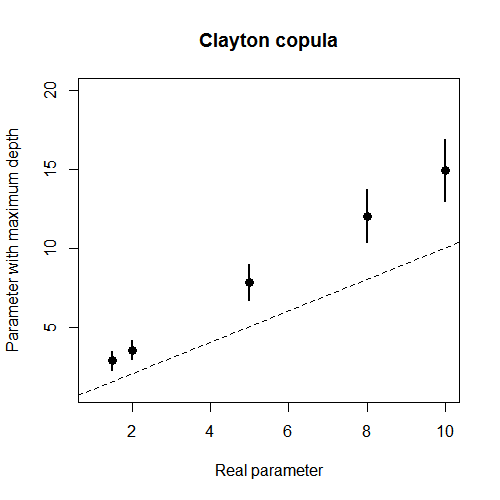
\includegraphics[height=6cm]{CopDepth_Clay.png}\\
		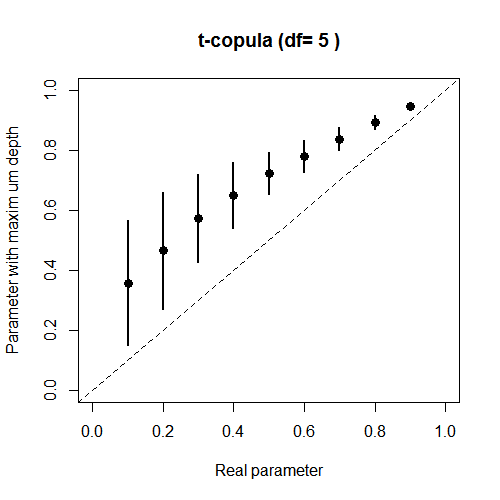
\includegraphics[height=6cm]{CopDepth_t5.png}
		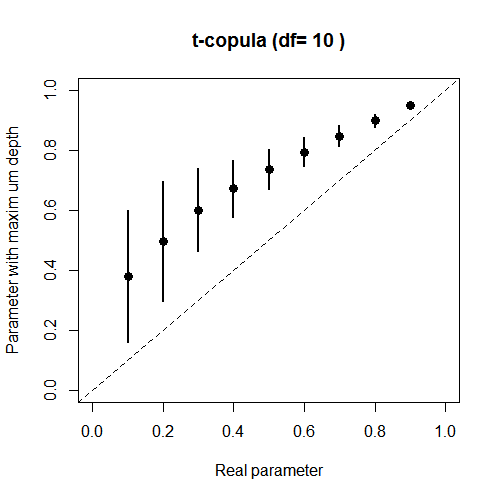
\includegraphics[height=6cm]{CopDepth_t10.png}
	\label{fig:fig1}
	\caption{Mean and standard deviations of simulated parameters with max depth}
\end{figure}
 
\subsection{Copula selection}Given data $\bfZ_1,...,\bfZ_n$ with $\bfZ_i=(X_i,Y_i)$ we first calculate the empirical copula of the data:
$$ C_e(u,v) = \frac{1}{n}\sum_{i=1}^n I(U_i\leq u, V_i\leq v)$$
where $\bfU = F_n(\bfX), \bfV = G_n(\bfY)$ are pseudosamples obtained from the data using marginal empirical distributions $F_n, G_n$ respectively. Given any copula $C$, we can calculate its distance from the empirical copula:
$$ d(C,C_e) = \sqrt{\sum_{i=1}^n\sum_{j=1}^n \left[C\left(\frac{i}{n},\frac{j}{n}\right) - C_e\left(\frac{i}{n},\frac{j}{n}\right)\right]^2} $$

For data on a pair of variables, we first calculate Kendall's $\tau$, and if it is $>0$ (or $<0$) consider Gaussian, $t$, (rotated) Clayton and (rotated) Gumbel copulae. ML and depth-based estimates are obtained for all copula parameters and then plugged into corresponding distributions. Finally for each method, ML and depth-based, the copula with least distance from the empirical copula as calculated above is chosen as the best-fitting copula. The degree of freedom parameter for both the methods is set as the one estimated by ML method.

\subsection{Constructing the graph}The Kendall's $\tau$ calculated from a bivariate dataset $(\bfZ_1,,,\bfZ_n)$ with $\bfZ_i=(X_i,Y_i); i = 1,...,n$ has an asymptotic normal distribution under the null hypothesis that $X$ and $Y$ are independent:
$$ \hat\tau \sim AN\left(0,\frac{2(2n+5)}{9n(n-1)}\right) $$
For a given multivariate data matrix, we consider a pair of variables, and given the sample size $n$ is large enough, test for independence between the variables using the asymptotic test above. Given that there is evidence of dependence, we attempt to choose the copula function that is the best fit to the data using the method outlined in 3.2, thus ending up with two copulas functions for ML and depth-based parameter estimations. Finally the whole process is repeated for all pairs of variables in the data.

\begin{algorithm}
\caption{Algorithm to obtain pairwise copula dependence network}
\begin{algorithmic}[1]
\Procedure{CopNetwork}{data matrix $\bfD\in \mathbb{R}^{n\times p}$}
\State Set $i=1,j=1$.
\State \emph{top}:
\State Set $\bfX=i^{th}$ column of $\bfD$, $\bfY=j^{th}$ column of $\bfD$.
\State Check for independence of $\bfX$ and $\bfY$ using test above.
\If {Independent}
	\State \textbf{goto} \emph{update}
\Else
	\If {Kendall's $\tau>0$}
		\State $S=$\{Gaussian, $t$, Clayton, Gumbel\}
	\Else
		\State $S=$\{Gaussian, $t$, rotated Clayton, rotated Gumbel\}
	\EndIf
	\State Select $C_{ij,M}\in S$ as the best fitting copula, parameter estimated by ML method.
	\State Select $C_{ij,D}\in S$ as the best fitting copula, parameter estimated by depth-based method.
\EndIf
\State \emph{update}:
\If {$j=p$}
	\If {$i=p$} \textbf{Stop}
	\Else \State Set $i\leftarrow i+1, j\leftarrow i$, \textbf{goto} \emph{top}
	\EndIf
\Else \State Set $j\leftarrow j+1$, \textbf{goto} \emph{top}
\EndIf

\EndProcedure
\end{algorithmic}
\end{algorithm}
\vspace{2cm}
\paragraph{}At the end of the algorithm we end up with two graphs, $\bfC_M$ and $\bfC_D$, giving best-fitting copulae, obtained by the two respective methods, for each pair of variables.

\section{Results}All analyses were performed in R version 3.0.2 \cite{R302}. We use the R packages \texttt{VineCopula} and \texttt{copula} for copula-related calculations. After obtaining two matrices $\bfC_M,\bfC_D$ we visualize the directional dependence structure by plotting it as a graph. Nodes correspond to  variables and edges between two nodes are colored according to the type of best-fitting copula between the variables.

\paragraph{}We now apply the methodology outlined above in two datasets from the UCI Machine Learning Repository (\url{http://archive.ics.uci.edu/ml}) to study the nature of dependence between variables.

\subsection{Breast Tissue data}The data consists of impedance measurements from 106 samples of freshly excised breast tissue. There are 9 measurement variables (I0, PA500, HFS, DA, Area, A/DA, Max IP, DR, P) and a class variable specifying the class of Breast Cancer the patient has (6 or 4 classes). For our analysis we ignore the class variable due to small sample sizes in each class and obtain the networks from the measurement variables only.

There are 28 significantly dependent variable pairs among 36 possible ones. Graphs indicate that variables except the two phase angle related variables: HFS and PA500, are all dependent on one another. Most of these dependencies are symmetric, and  heavy-tailed ($t$-copula) as per the ML method, but light-tailed as per the depth-based method (Figure 2).

\begin{figure}[H]
	\centering
		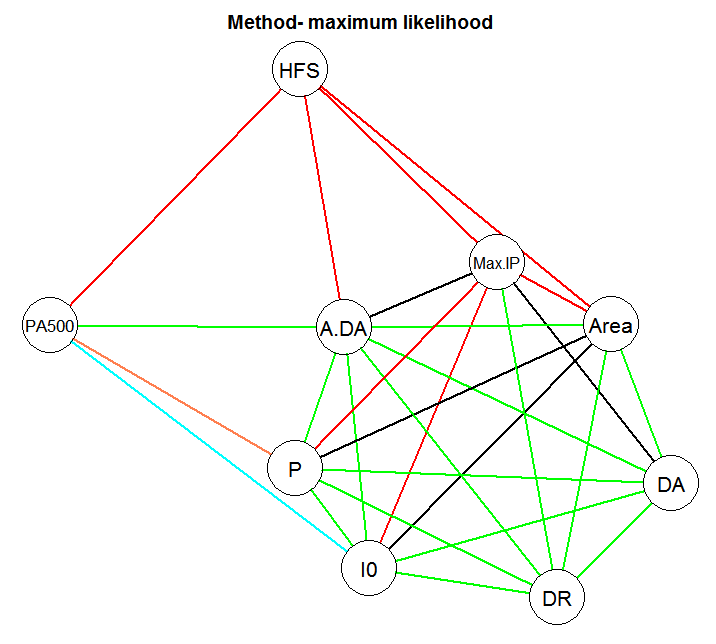
\includegraphics[height=6cm]{cancer_graph_ml.png}\\
		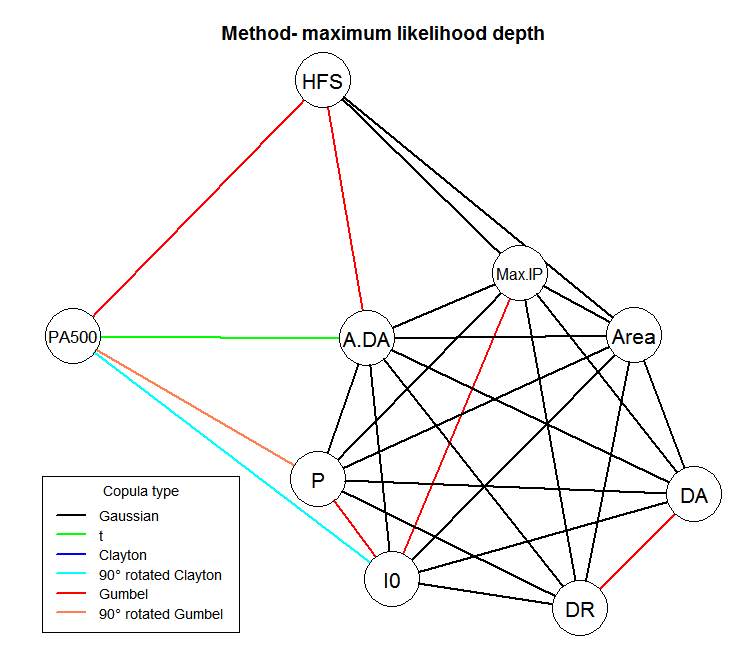
\includegraphics[height=6cm]{cancer_graph_md.png}
	\label{fig:fig2}
	\caption{Graph of Breast Cancer variables obtained by best-fitting (top) ML copula, (Bottom) MLD copula}
\end{figure}

\begin{table}[h]\centering
    \begin{tabular}{l|l}
    \hline
    Variable name & Description          \\\hline
    I0       & Impedivity (ohm) at zero frequency                                \\
    PA500    & Phase angle at 500 KHz                                            \\
    HFS      & High-frequency slope of phase angle                               \\
    DA       & Impedance distance between spectral ends                          \\
    AREA     & Area under spectrum                                               \\
    A/DA     & Area normalized by DA                                             \\
    MAX IP   & Maximum of the spectrum                                           \\
    DR       & Distance between I0 and real part of the maximum frequency point  \\
    P        & Length of the spectral curve                                      \\\hline
    \end{tabular}
    \caption{Description of measurement variables in Breast Cancer data}
\end{table}

\subsection{Cardiotocography data}This dataset has measurements relating to 2126 fetal cardiotocograms. There are 21 predictor variables, and a class variable describing fetal state (N=normal, S=suspect, P=pathologic). The descriptions of variables are given in the appendix. There are 3 types of variables:
\begin{enumerate}
\item Variables 1-7 give numerical measurements, like number of fetal movements, uterine contractions etc (Group A),
\item Variables 8-11 are about variability of cardiograms with respect to time (Group B),
\item Variables 12-21 give measurements of heart-rate histograms, like max, min, mean, median etc. (Group C)
\end{enumerate}
DS, the sixth variable has most of its values set at 0, so we exclude it from our analysis.

\subsubsection{Variable group-specific analysis}
Over 90\% of connections between the 20 variables (176 among 190 possible) are found significant in the initial screening for dependence. Hence instead of plotting the graph we analyze the dependence structures within and between the 3 variable groups. There are 3 within-group ($AA, BB, CC$) and 3 between-group ($AB, AC, BC$) interactions. The type of copulas fit by ML method for each of these 6 interactions are listed in Table 2.
%\begin{enumerate}
%\item All the pairwise dependences within numerical variables are assymetric.
%\item 
%\end{enumerate}

\begin{table}[ht]\centering
    \begin{tabular}{|c||c|c|c|c|c|c|c|}
    \hline
    Interaction & Independent & Gaussian & $\quad t\quad$ & Clayton & rot. Clayton & Gumbel & rot. Gumbel \\ \hline
    AA                  & 2           & 0        & 0 & 7       & 1               & 0      & 5              \\
    BB                  & 1           & 2        & 1 & 0       & 1               & 0      & 1              \\
    CC                  & 2           & 11       & 9 & 2       & 7               & 5      & 9              \\ \hline\hline
    AB                  & 1           & 4        & 3 & 2       & 11              & 1      & 2              \\
    AC                  & 3           & 16       & 2 & 16      & 18              & 2      & 3              \\
    BC                  & 5           & 7        & 3 & 7       & 11              & 2      & 5              \\ \hline
    \end{tabular}
    \caption{Summary of best-fitting copulae for within (Top 3) and between (bottom 3) group dependencies in CTG data}
\end{table}

\subsubsection{Dependence structure for different fetal classes} We also compare between the within-group dependencies for the 3 fetal classes. Figs 3 and 4 outline differences in groups A and B for 3 sample classes. For variable group C, the summary of copulae fit between the 45 variable-pairs is summarized in table 3. Highlights include a high amount of independence in suspect class and high asymetric dependencies in pathologic class.

\begin{table}[h]\centering
    \begin{tabular}{|c||c|c|c|c|c|c|c|}
    \hline
    Sample class & Independent & Gaussian & $\quad t\quad$ & Clayton & rot. Clayton & Gumbel & rot. Gumbel \\ \hline
    Normal & 4 & 13 & 8 & 4 & 5 & 7 & 4 \\
    Suspect & 11 & 8 & 8 & 3 & 3 & 10 & 2 \\
    Pathologic & 3 & 9 & 2 & 2 & 11 & 7 & 11 \\ \hline
    \end{tabular}
    \caption{Best-fitting copulae by ML method for group C variables in CTG data}
\end{table}

\begin{figure}[H]
	\centering
		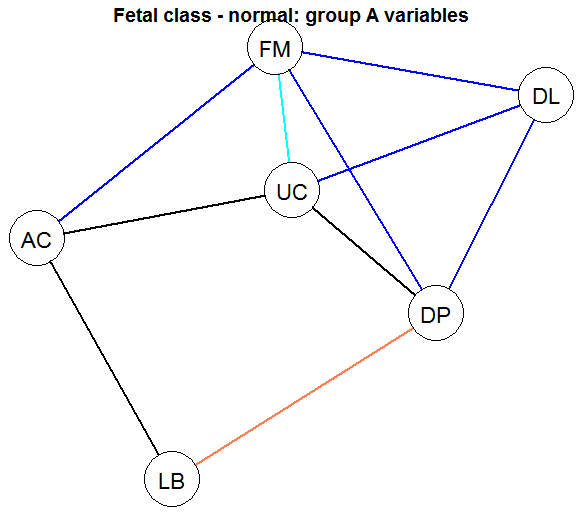
\includegraphics[height=7cm]{ctgplot_1a.png}\\
		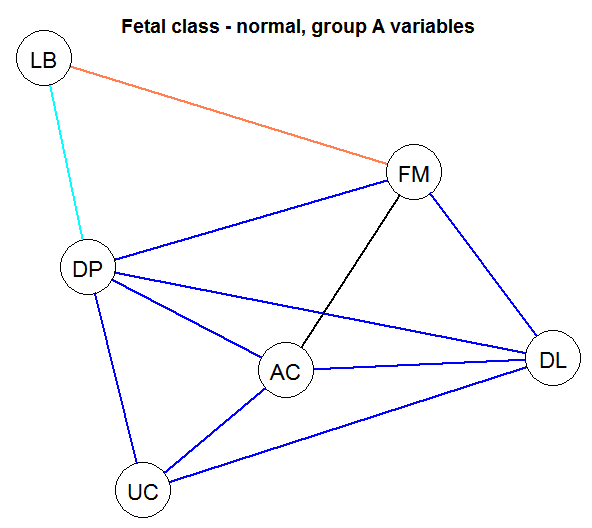
\includegraphics[height=7cm]{ctgplot_2a.png}\\
		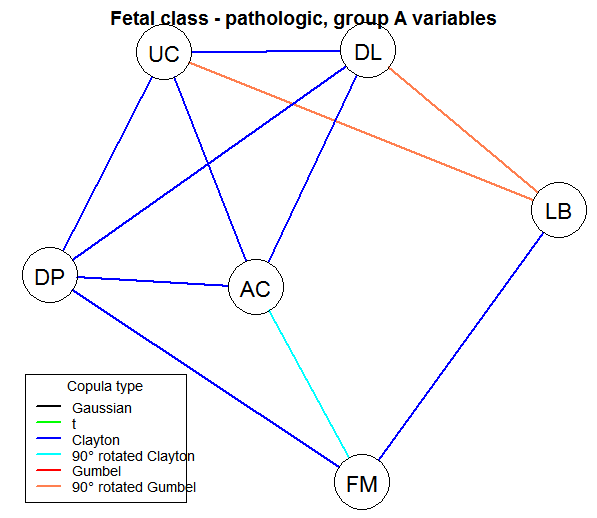
\includegraphics[height=7cm]{ctgplot_3a.png}
	\label{fig:fig2}
	\caption{Graph of group A variables for 3 classes}
\end{figure}


\begin{figure}[H]
	\centering
		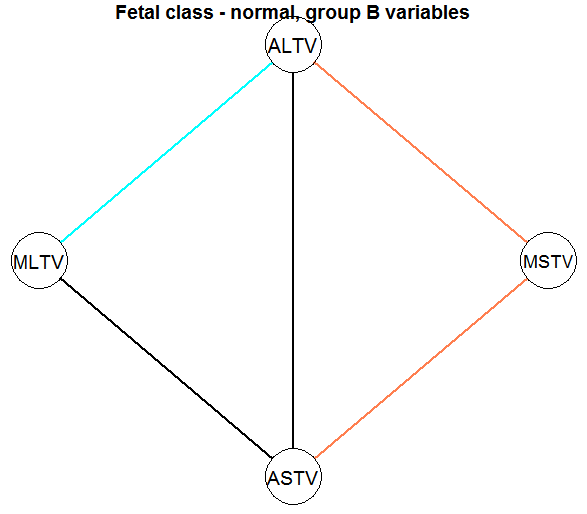
\includegraphics[height=7cm]{ctgplot_1b.png}\\
		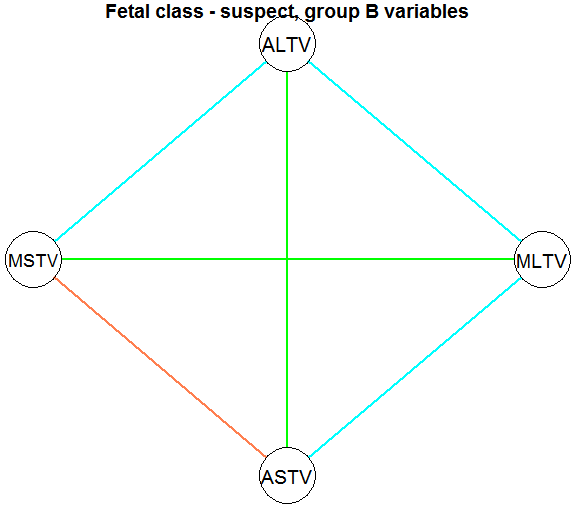
\includegraphics[height=7cm]{ctgplot_2b.png}\\
		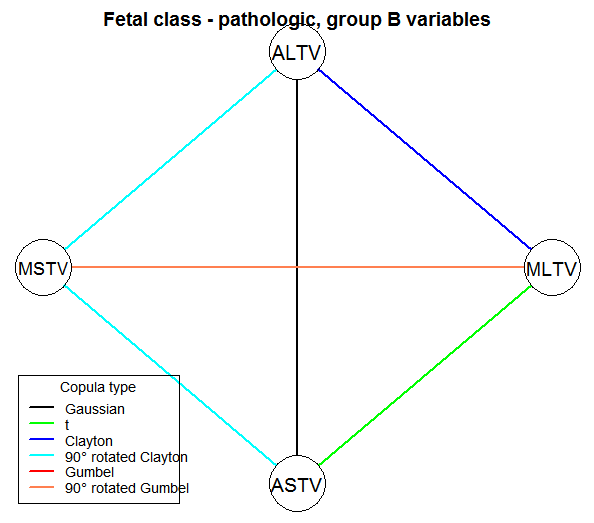
\includegraphics[height=7cm]{ctgplot_3b.png}
	\label{fig:fig2}
	\caption{Graph of group B  variables for 3 classes}
\end{figure}

%\begin{table}[!h]
%\begin{center}
%\begin{tabular}[c]{|c|c||c|c|c|c|c|c|c|}\hline
% & & \multicolumn{7}{c|}{Method of analysis (powers in percentage)}\\\cline{3-9}
%\begin{large} $p$ \end{large} &\begin{large} $d$ \end{large} & All & All & Omit affected & Omit treated & Treatment & Constant & Non-parametric \\
% & (mm Hg) & underlying & observed & subjects & subjects & as covariate & adjustment & adjustment\\\hline\hline
% & 10 & 44.7 & 42.4 & 29.9 & 31.7 & 29.0 & 44.3 & 41.7\\\cline{2-9}
% & 15 & 81.2 & 79.1 & 60.8 & 68.6 & 59.5 & 80.9 & 79.8\\\cline{2-9}
%\begin{large} \textbf{0.1} \end{large} & 20 & 97.3 & 97.0 & 86.1 & 89.9 & 85.9 & 97.3 & 97.1\\\cline{2-9}
% & 25 & 99.7 & 99.7 & 97.5 & 98.1 & 97.0 & 99.7 & 99.7\\\cline{2-9}
% & 30 & 100.0 & 100.0 & 99.7 & 99.7 & 99.5 & 100.0 & 100.0\\\cline{2-9}\hline\hline
%
% & 10 & 80.3 & 79.1 & 53.3 & 65.9 & 56.6 & 80.0 & 78.0\\\cline{2-9}
% & 15 & 98.9 & 97.8 & 90.2 & 93.9 & 91.6 & 98.6 & 98.8\\\cline{2-9}
%\begin{large} \textbf{0.3} \end{large} & 20 & 100.0 & 100.0 & 99.3 & 99.8 & 99.7 & 100.0 & 100.0\\\cline{2-9}
% & 25 & 100.0 & 100.0 & 100.0 & 100.0 & 100.0 & 100.0 & 100.0\\\cline{2-9}
% & 30 & 100.0 & 100.0 & 100.0 & 100.0 & 100.0 & 100.0 & 100.0\\\cline{2-9}\hline\hline
%
% & 10 & 86.0 & 84.3 & 65.5 & 74.0 & 70.4 & 86.0 & 83.2\\\cline{2-9}
% & 15 & 99.7 & 98.8 & 95.2 & 97.6 & 96.9 & 99.7 & 99.5\\\cline{2-9}
%\begin{large} \textbf{0.5} \end{large} & 20 & 100.0 & 100.0 & 99.9 & 100.0 & 100.0 & 100.0 & 100.0\\\cline{2-9}
% & 25 & 100.0 & 100.0 & 100.0 & 100.0 & 100.0 & 100.0 & 100.0\\\cline{2-9}
% & 30 & 100.0 & 100.0 & 100.0 & 100.0 & 100.0 & 100.0 & 100.0\\\cline{2-9}\hline
%\end{tabular}
%\caption{Powers obtained by different methods for $\delta' = 1$}
%\end{center}
%\end{table}

\section{Conclusion}In the above sections we have outlined a distribution-free method to analyze the nature of dependencies between pairs of variables in a multivariate dataset. Applications on two real datasets are also done.

\paragraph{}We aim to formulate a robust framework for estimating directional dependencies that can extend the applicability domain of copula functions. Further work on this direction includes using conditional bivariate copula for each variable-pair to eliminate effect of other variables. We also plan to do detailed simulation studies to compare between the two methods of copula parameter estimation, as well as analyze genetic data and compare the methodology with other known methods.

\section*{Acknowledgment}I thank my adviser Prof. Snigdhansu Chatterjee for his guidance and valuable inputs throughout the project.

\bibliographystyle{acm}
\bibliography{depth}

\newpage
\section*{Appendix 1: Calculating unbiased estimator of $\rho$ from MLDE for $t$-copula}
The true parameter value $\rho$ is related to the MLDE $\hat\rho_d$ as follows:
$$ \rho = \begin{cases}
\sign(\hat\rho_d)\left[c_3|\hat\rho_d|^3 + c_2|\hat\rho_d|^2 + c_1|\hat\rho_d| + c_0\right]
&\mbox{if } |\hat\rho_d| > \rho_0\\ 0 &\mbox{if }|\hat\rho_d| \leq \rho_0 
\end{cases}$$
where the coefficients $c_0, ... , c_3$ and the cutoff point $\rho_0$ are chosen from the row in Table 4 corresponding to the df of $t$-copula.
\begin{table}[h]\centering
    \begin{tabular}{c|ccccc}
    \hline
     df & $\quad c_0\quad$      & $\quad c_1\quad$     & $\quad c_2\quad$     & $\quad c_3\quad$     & $\rho_0$  \\ \hline
    3   & -0.1272 & 0.5657 & 0.2685 & 0.3057 & 0.2272 \\
    4   & -0.1305 & 0.5061 & 0.3038 & 0.3343 & 0.2392 \\
    5   & -0.135  & 0.4826 & 0.2976 & 0.3686 & 0.2562 \\
    6   & -0.1419 & 0.5058 & 0.2062 & 0.4456 & 0.2693 \\
    7   & -0.1066 & 0.285  & 0.5389 & 0.2971 & 0.2853 \\
    8   & -0.1167 & 0.3246 & 0.4431 & 0.3649 & 0.2797 \\
    9   & -0.1075 & 0.2856 & 0.4717 & 0.3665 & 0.2881 \\
    10  & -0.1192 & 0.3207 & 0.4251 & 0.3889 & 0.2835 \\
    11  & -0.1575 & 0.5098 & 0.1136 & 0.5508 & 0.2956 \\
    12  & -0.146  & 0.4432 & 0.2057 & 0.5142 & 0.3079 \\
    13  & -0.1447 & 0.4199 & 0.2474 & 0.494  & 0.3038 \\
    14  & -0.1338 & 0.3706 & 0.3035 & 0.4758 & 0.3008 \\
    15  & -0.1334 & 0.3411 & 0.3674 & 0.4407 & 0.3186 \\
    16  & -0.1351 & 0.3739 & 0.2754 & 0.503  & 0.2964 \\
    17  & -0.1221 & 0.3006 & 0.3854 & 0.4526 & 0.2945 \\
    18  & -0.1106 & 0.2404 & 0.4772 & 0.4099 & 0.3101 \\
    19  & -0.1503 & 0.4428 & 0.1508 & 0.5744 & 0.2966 \\
    20  & -0.1636 & 0.5092 & 0.0411 & 0.6321 & 0.3135 \\
    21  & -0.1385 & 0.3805 & 0.2286 & 0.5483 & 0.3192 \\
    22  & -0.1429 & 0.3927 & 0.2227 & 0.5457 & 0.3042 \\
    23  & -0.1451 & 0.3991 & 0.2159 & 0.5477 & 0.3115 \\
    24  & -0.1265 & 0.3132 & 0.3345 & 0.4968 & 0.3179 \\
    25  & -0.136  & 0.3428 & 0.2983 & 0.5128 & 0.32   \\
    26  & -0.1141 & 0.2425 & 0.4325 & 0.4568 & 0.3115 \\
    27  & -0.1521 & 0.4334 & 0.1469 & 0.59   & 0.3127 \\
    28  & -0.1582 & 0.4675 & 0.0917 & 0.6171 & 0.3233 \\
    29  & -0.1521 & 0.4485 & 0.1003 & 0.6222 & 0.3176 \\
    30  & -0.1519 & 0.4504 & 0.0953 & 0.625  & 0.3119 \\\hline
    \end{tabular}
    \caption{Table for $t$ copula unbiased estimator calculation}
\end{table}

\section*{Appendix 2: Description of variables in Cardiotocography data}
\begin{table}[H]\centering
    \begin{tabular}{l|l}
    \hline
    Variable name & Description (FHR = Fetal Heart Rate)                     \\ \hline
    LB            & FHR baseline (beats per minute)                          \\
    AC            &  \# of accelerations per second                \\
    FM            & \# of fetal movements per second               \\
    UC            & \# of uterine contractions per second          \\
    DL            & \# of light decelerations per second           \\
    DS            & \# of severe decelerations per second          \\
    DP            & \# of prolongued decelerations per second      \\ \hline
    ASTV          & Percentage of time with abnormal short term variability  \\
    MSTV          & Mean value of short term variability                     \\
    ALTV          & Percentage of time with abnormal long term variability   \\
    MLTV          & Mean value of long term variability                      \\ \hline
    Width         & Width of FHR histogram                                   \\
    Min           & Minimum of FHR histogram                                 \\
    Max           & Maximum of FHR histogram                                 \\
    Nmax          & \# of histogram peaks                          \\
    Nzeros        & \# of histogram zeros                          \\
    Mode          & Histogram mode                                           \\
    Mean          & Histogram mean                                           \\
    Median        & Histogram median                                         \\
    Variance      & Histogram variance                                       \\
    Tendency      & Histogram tendency                                       \\ \hline
    \end{tabular}
    \caption{Description of variables in Cardiotocography data}
\end{table}

\end{document} 
